\documentclass[runningheads]{llncs}
% MICCAI submission draft: Springer LNCS, 8 pages of content plus up to 2 of
% references (2026 rules; check the 2027 call when it is published).
% Double-blind: no author names, no identifying repository links.
\usepackage[T1]{fontenc}
\usepackage{lmodern}
\usepackage{microtype}
\usepackage{amsmath}
\usepackage{booktabs}
\usepackage{graphicx}
\usepackage{xcolor}
\usepackage{hyperref}
\graphicspath{{../../figures/}}

% Anything that waits on the registered grid or a later run.
\newcommand{\pending}[1]{\textcolor{red!70!black}{[\textbf{pending:} #1]}}
\newcommand{\todo}[1]{\textcolor{orange!80!black}{[\textbf{todo:} #1]}}

\begin{document}

\title{What a Pre-Registered Study Shows About Type Conditioning,
Label-Aware Augmentation and Split Protocol in 2D Brain-Tumour Segmentation}
\titlerunning{Pre-Registered Study of 2D Brain-Tumour Segmentation}
\author{Anonymized Authors}
\authorrunning{Anonymized Authors}
\institute{Anonymized Institutions}

\maketitle

\begin{abstract}
\pending{written last, after the H2--H4 results. At most 250 words.}
\keywords{Segmentation \and Pre-registration \and Data leakage \and Data augmentation}
\end{abstract}

\section{Introduction}

The Cheng dataset~\cite{chengdata,cheng2015} contains 3064 T1-weighted
contrast-enhanced MRI slices from 233 patients with meningioma, glioma or
pituitary tumours. Every slice carries a tumour mask, a type label and a patient
identifier. Released for type classification~\cite{cheng2015}, it has become a
common 2D segmentation benchmark. Two ideas recur in recent work on it: using the
tumour type to help segmentation, and label-aware intensity augmentation that
remaps tumour and background separately~\cite{yurdakul2026}.

We tested both in a pre-registered study. The analysis plan, including a
\emph{baseline credibility gate}, was committed before any run finished.
\todo{introduction arc, after results: (i) does type conditioning help;
(ii) the gate failing and what the split unit does to the numbers;
(iii) what label-aware augmentation teaches the network.}

\noindent\textbf{Contributions.} \todo{final list after results. Candidates:
a pre-registered null or negative result for type-conditioned decoding; a
like-for-like measurement of the split-unit effect and of the variance collapse it
causes; a measured label shortcut in mask-dependent augmentation.}

\section{Related Work}
\label{sec:related}

\noindent\textbf{Evaluation on the Cheng benchmark.}
Studies differ in whether they split by patient or by slice. Several give only
slice or image counts~\cite{gupta2023,rai2024,preetha2025}, and Preetha et al.\
use a 90:10 split of slices without cross-validation~\cite{preetha2025}. Others
split by patient~\cite{avazov2024,yurdakul2026}. Yurdakul et al.\ benchmark
fourteen architectures under stratified group five-fold cross-validation at
patient level. Dice ranges from 84.0 to 89.6, and a plain U-Net scores
$84.1\pm1.6$~\cite[Table~2]{yurdakul2026}.

\noindent\textbf{Leakage, aggregation and variance.}
Slice-level splits of brain MRI inflated 2D CNN classification accuracy by
29--55\%, and reached about 96\% on randomly labelled data~\cite{yagis2021}.
Leakage affects at least 294 papers across 17 fields~\cite{kapoor2023}, and data
and evaluation choices bias medical-imaging results more broadly~\cite{varoquaux2022}.
Aggregation choices change challenge winners~\cite{maierhein2018}, metric choice
should follow from the problem~\cite{maierhein2024}, and benchmark variance is
large enough to produce spurious improvements~\cite{bouthillier2021}.

\noindent\textbf{Type conditioning.}
FiLM conditions features through a learned per-channel scale and
shift~\cite{perez2018}. On this dataset, segmentation and classification have
usually been parallel heads on a shared encoder~\cite{rai2024}. We instead
condition the decoder on the type posterior. \todo{search for prior
class-conditioned decoders in medical segmentation before claiming novelty.}

\noindent\textbf{B\'ezier intensity augmentation and shortcuts.}
Models Genesis introduced monotonic cubic B\'ezier intensity
transforms~\cite{zhou2021genesis}. They have since been used for single-source
domain generalisation~\cite{zhou2022style}. SLAug~\cite{su2023slaug} and
Yurdakul et al.~\cite{yurdakul2026} make them label-aware by transforming
regions cropped with the ground-truth mask. A network uses any cue that separates
the training labels, whether or not it exists at test time~\cite{geirhos2020}.
A mask-dependent transform can create exactly such a cue.

\section{Methods}
\label{sec:methods}

\noindent\textbf{Pre-registration.}
Hypotheses, outcomes, statistics, equivalence margin, decision rules, stopping
rule and the credibility gate were committed on 14 September 2026, before any
run completed. Later decisions appear only as dated deviations, and the analyses
they add are labelled exploratory. \todo{anonymised repository link
(e.g.\ anonymous.4open.science) and registration commit hash.}

\noindent\textbf{Data and splits.}
Stratified group five-fold cross-validation at patient ID (seed 42), with a
patient-disjoint validation set carved from each training portion (70/10/20).
For the protocol analysis only, a slice-level five-fold split is drawn with the
same seed. Under it, 224 of 233 patients span more than one fold.

\noindent\textbf{Models.}
A U-Net (31.0M parameters) is the baseline. The conditioned U-Net adds a type
head on the bottleneck (average pooling, dropout 0.1, linear). Each decoder stage
output $x$ becomes $x(1+\gamma)+\beta$, with $\gamma,\beta$ a linear projection
of a three-dimensional condition vector. The projection is zero-initialised, so
the conditioned network starts identical to the baseline. The condition is the
softmax type posterior (\emph{predicted}) or the one-hot true type
(\emph{oracle}). Loss: Dice+BCE (weight 0.5) plus type cross-entropy (weight 0.2).

\noindent\textbf{Augmentation arms.}
All arms share geometric augmentation (horizontal flip, rotation $\pm15^\circ$,
scale $\pm10\%$), drawn identically item by item across arms. \emph{Standard}
adds nothing. \emph{Global} remaps the image through one random cubic B\'ezier
curve. \emph{Region} remaps tumour and background, as given by the ground-truth
mask, through two independent curves. Curves are monotonic with probability 0.5,
and otherwise order-reversing. As registered, both B\'ezier arms apply to every
image with control points drawn from the full unit square. Yurdakul et al.\ use
probability 0.5, a deviation bound of 0.5 and boundary smoothing~\cite{yurdakul2026}.

\noindent\textbf{Training and statistics.}
Input $192\times192$, effective batch 16, AdamW (learning rate $10^{-4}$, weight
decay $10^{-2}$), cosine schedule, at most 150 epochs, early stopping on
validation Dice with patience 20. Initialisation is seeded per fold, shared across
arms. Co-primary outcomes are slice-averaged and patient-averaged Dice. Each of
four hypotheses is a paired comparison over five folds: H1 predicted vs.\ U-Net,
H2 oracle vs.\ predicted, H3 region vs.\ standard, H4 region vs.\ global. We
report paired $t$-tests with 95\% CIs, Holm-corrected ($m=4$), and TOST against
a registered margin of $\pm0.005$ Dice.

\section{Results}

\noindent\textbf{Baseline and credibility gate.}
The U-Net reached $0.7719\pm0.0164$ slice-averaged Dice ($0.7699\pm0.0286$
patient-averaged), 6.9 points below the 84.1 reported under a patient-level
split~\cite{yurdakul2026}. The gate failed and the gap remains unexplained.
Weight decay ($10^{-2}$ here, $10^{-4}$ in the source) is the main untested
difference. \pending{exploratory five-fold run at weight decay $10^{-4}$.}

\noindent\textbf{Split protocol.}
Retraining the same model on a slice-level split (Table~\ref{tab:protocol})
adds 4.3--5.1 Dice points. The between-fold standard deviation shrinks
3--8$\times$, because the folds no longer sample patients. The gain is
concentrated in glioma ($0.663\to0.734$; zero-Dice slices 133$\to$88 of 1426)
and does not grow with training length ($r=-0.21$, $n=5$). Fold 0 alone
understated the five-fold effect by three points.

\begin{table}[t]
\centering
\caption{One U-Net under two split units, five folds each (unpaired).}
\label{tab:protocol}
\begin{tabular}{@{}lcccc@{}}
\toprule
aggregation & patient-disjoint & slice-level & difference & sd ratio\\
\midrule
slice-averaged & $0.7719\pm0.0164$ & $0.8152\pm0.0035$ & $+0.0433$ & $4.8\times$\\
pooled & $0.7846\pm0.0165$ & $0.8358\pm0.0054$ & $+0.0511$ & $3.0\times$\\
patient-averaged & $0.7699\pm0.0286$ & $0.8152\pm0.0035$ & $+0.0453$ & $8.3\times$\\
\bottomrule
\end{tabular}
\end{table}

\begin{figure}[t]
\centering
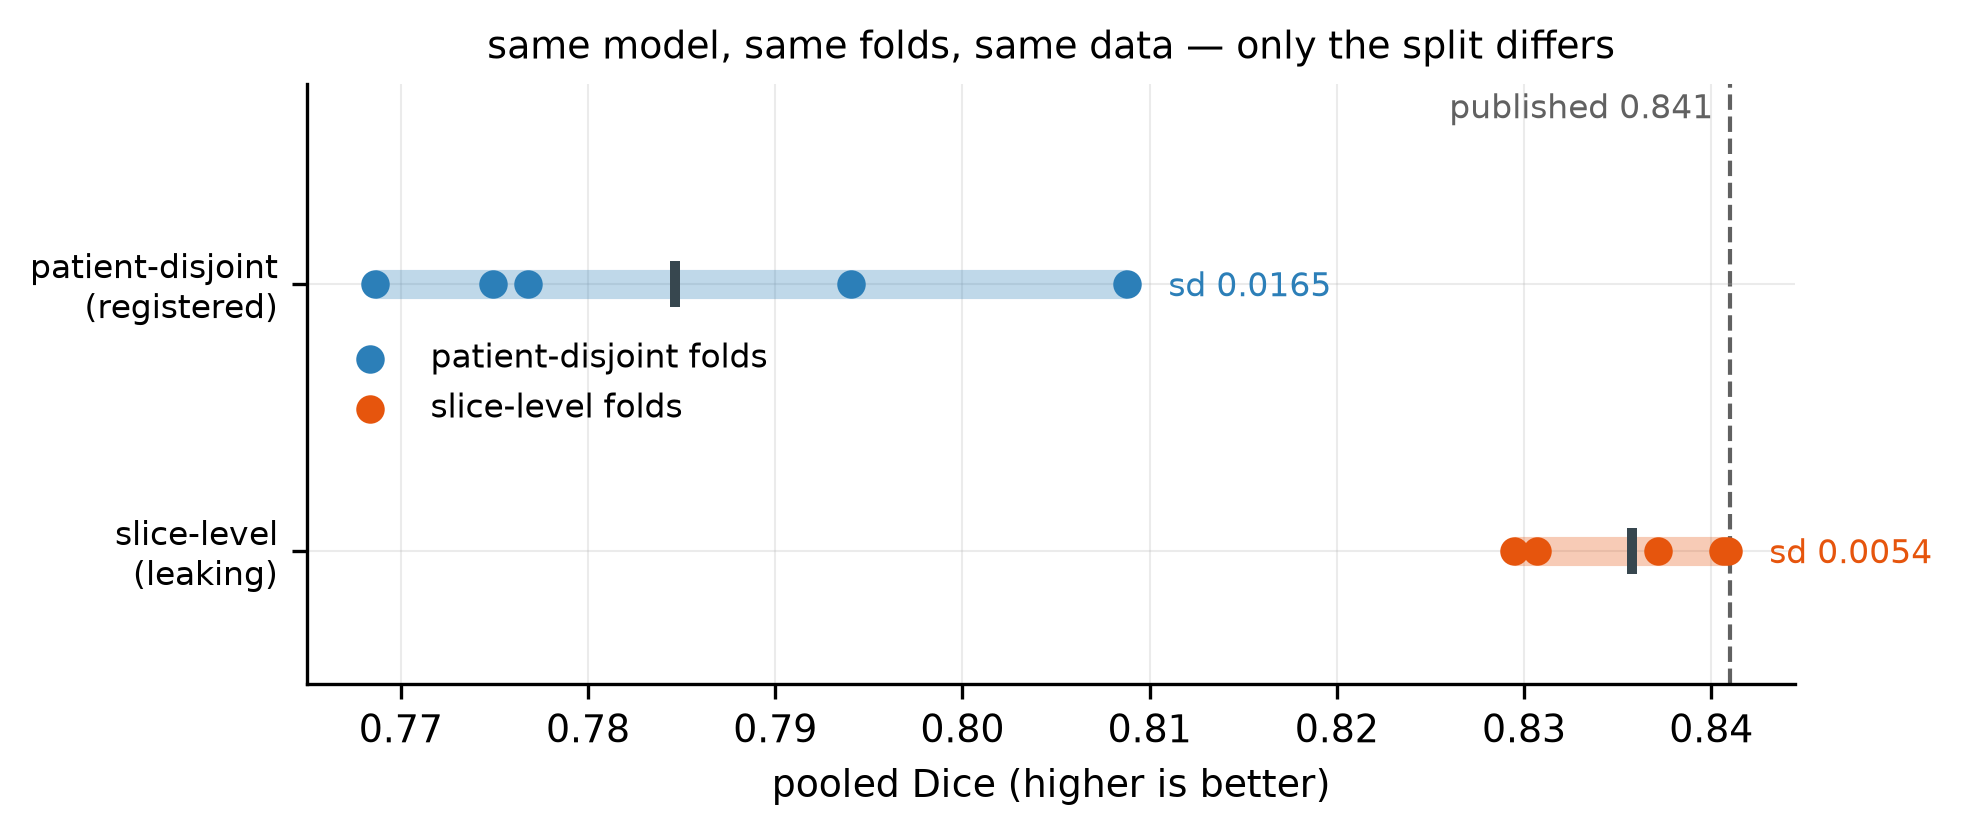
\includegraphics[width=0.49\linewidth]{protocol.png}\hfill
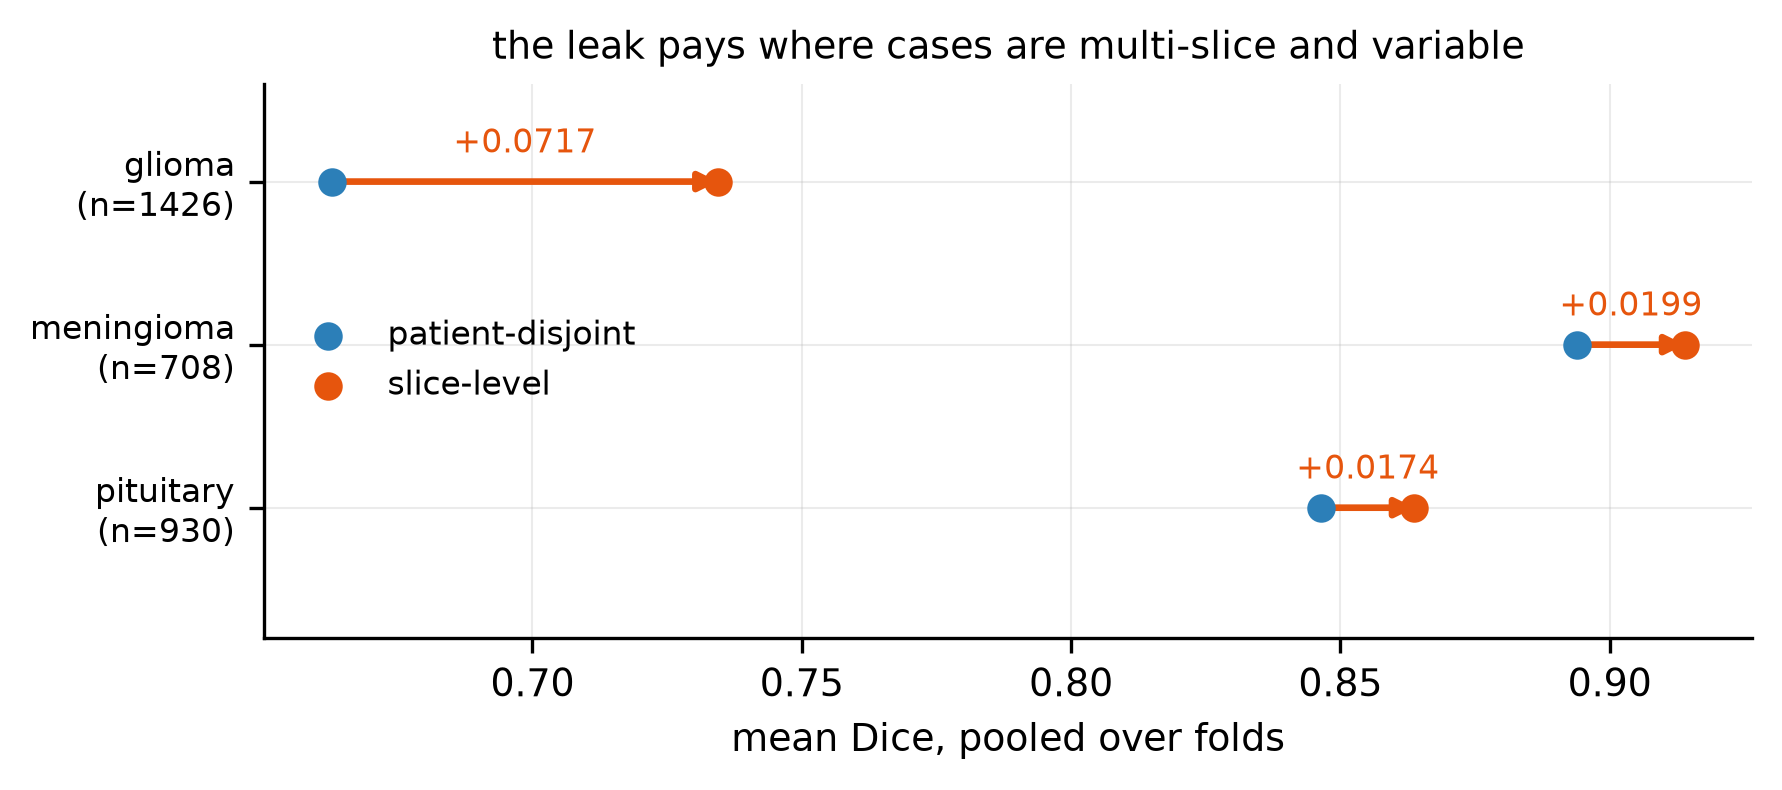
\includegraphics[width=0.49\linewidth]{protocol_by_type.png}
\caption{Left: per-fold pooled Dice under both split units. Right: by tumour type.}
\label{fig:protocol}
\end{figure}

\noindent\textbf{H1: predicted-type conditioning.}
Table~\ref{tab:hyp}. H1 is inconclusive under the registered rules. The estimate
is negative on both co-primary outcomes and for every tumour type, although the
type head reaches 93.8\% accuracy.

\begin{table}[t]
\centering
\caption{Registered contrasts over five paired folds. $p$ before Holm correction.}
\label{tab:hyp}
\begin{tabular}{@{}llccc@{}}
\toprule
& outcome & difference [95\% CI] & $p$ & TOST $p$\\
\midrule
H1 & slice-avg.\ Dice & $-0.0088\ [-0.025,+0.008]$ & 0.21 & 0.72\\
   & patient-avg.\ Dice & $-0.0147\ [-0.031,+0.001]$ & 0.063 & 0.92\\
H2 & slice-avg.\ Dice & \pending{} & & \\
   & patient-avg.\ Dice & \pending{} & & \\
H3 & slice-avg.\ Dice & \pending{} & & \\
   & patient-avg.\ Dice & \pending{} & & \\
H4 & slice-avg.\ Dice & \pending{} & & \\
   & patient-avg.\ Dice & \pending{} & & \\
\bottomrule
\end{tabular}
\end{table}

\noindent\textbf{H2: oracle conditioning.}
\pending{if the oracle also fails to beat the U-Net, type information does not
help this decoder at all, not merely imperfect predictions.}

\noindent\textbf{H3 and H4: region-wise augmentation.}
Before folds 1--4 ran, we measured how strongly each arm marks the label
boundary. Over 100 training slices, the median intensity step across the tumour
boundary, divided by the image standard deviation, was 0.39 (standard), 0.33
(global) and 1.55 (region), exceeding one standard deviation on 8\%, 3\% and 62\%
of slices. On fold 0 the region arm reached a training loss of 0.014 but a test
Dice of 0.5746, against 0.7914 for standard. This measurement and the prediction
that H3 and H4 would be negative were recorded before the remaining folds.
\pending{five-fold H3 and H4; corrected-arm result if run.}

\section{Discussion and Conclusion}
\pending{after results: why type information does or does not help; what the
split effect means for comparing papers on this benchmark; label-aware
augmentation as a shortcut and the settings that limit it; the open 84.1 gap.}

\noindent\textbf{Limitations.}
One dataset, one architecture family, one seed per fold and five folds, so
intervals are wide. The protocol comparison is unpaired. The registered region arm
perturbs more often and more strongly than the source method~\cite{yurdakul2026},
so a negative H3 describes this implementation, not theirs.

\bibliographystyle{splncs04}
\bibliography{../journal/refs}

\end{document}
